\documentclass[12pt,fleqn,answers]{exam}
\usepackage{amssymb}
\usepackage[intlimits]{amsmath}
\usepackage{epsfig}
\usepackage{upgreek}
\usepackage[super]{nth}
\usepackage[colorlinks=true,linkcolor=black,anchorcolor=black,citecolor=black,filecolor=black,menucolor=black,runcolor=black,urlcolor=black]{hyperref}
\usepackage[letterpaper, margin=0.75in]{geometry}
\addpoints
\boxedpoints
\pointsinmargin
\pointname{pts}
\usepackage{tikz}
\usepackage{tkz-euclide}
\usetikzlibrary{shapes.geometric}
\usetikzlibrary{calc}
\usepackage[final]{microtype}
\frenchspacing
\usepackage[american]{babel}
\usepackage[T1]{fontenc}
\usepackage[]{fourier}
\usepackage{isomath}
\usepackage{upgreek,amsmath}
\usepackage{graphicx}

\newcommand{\dotprod}{\, {\scriptzcriptztyle\stackrel{\bullet}{{}}}\,}

\newcommand{\reals}{\mathbf{R}}
\newcommand{\lub}{\mathrm{lub}} 
\newcommand{\glb}{\mathrm{glb}} 
\newcommand{\complex}{\mathbf{C}}
\newcommand{\dom}{\mbox{dom}}
\newcommand{\range}{\mbox{range}}
\newcommand{\cover}{{\mathcal C}}
\newcommand{\integers}{\mathbf{Z}}
\newcommand{\vi}{\, \mathbf{i}}
\newcommand{\vj}{\, \mathbf{j}}
\newcommand{\vk}{\, \mathbf{k}}
\newcommand{\bi}{\, \mathbf{i}}
\newcommand{\bj}{\, \mathbf{j}}
\newcommand{\bk}{\, \mathbf{k}}
\DeclareMathOperator{\Arg}{\mathrm{Arg}}
\DeclareMathOperator{\Ln}{\mathrm{Ln}}
\newcommand{\imag}{\, \mathrm{i}}

\usepackage{graphicx}
\usepackage{color}
%\shadedsolutions
%\definecolor{SolutionColor}{rgb}{1,0.72,0.46} %{0.8,0.9,1}
\newcommand\AM{\textsc{am}}
\newcommand\PM{\textsc{pm}}
     
\newcommand{\quiz}{16}
\newcommand{\term}{Fall}
\newcommand{\due}{Tuesday 24 October 13:20}
\newcommand{\class}{MATH 202, Fall \the\year}
\begin{document}
\large
\vspace{0.1in}
\noindent\makebox[3.0truein][l]{\textbf{\class}}
\textbf{Name:} \hrulefill \\
\noindent \makebox[3.0truein][l]{\textbf{In class work  \quiz}}
\textbf{Row and Seat}:\hrulefill\\

\noindent \emph{“The place to improve the world is first in one's own heart and head and hands, and then work outward from there.”} \hfill 
   \hfill {\sc Robert M. Pirsig}


\noindent  In class work  \textbf{\quiz}  has questions \textbf{1} 
through  \textbf{\numquestions} \/ with a total of 
\textbf{\numpoints\/} points. Turn in your work at the end of class 
\emph{on paper}. This assignment is due \emph{\due}.

\vspace{0.1in}



\begin{questions} 

\question Define a function $F$ by $F(x) = \frac{\ln(x)}{\left(\frac{4}{3}\right)^x}$.

\begin{parts}

\part [1] Use Desmos to graph $y  = F(x)$ for $ 2 \leq x \leq  15$. Reproduce the graph here. Based on the graph, what is your
guess for the numeric value of $\displaystyle \lim_{x \to \infty}  \frac{\ln(x)}{\left(\frac{4}{3}\right)^x}$?


    \begin{solution}[1.50in] The graph indicates that  $\displaystyle \lim_{x \to \infty}  \frac{\ln(x)}{\left(\frac{4}{3}\right)^x} = 0$.
    
        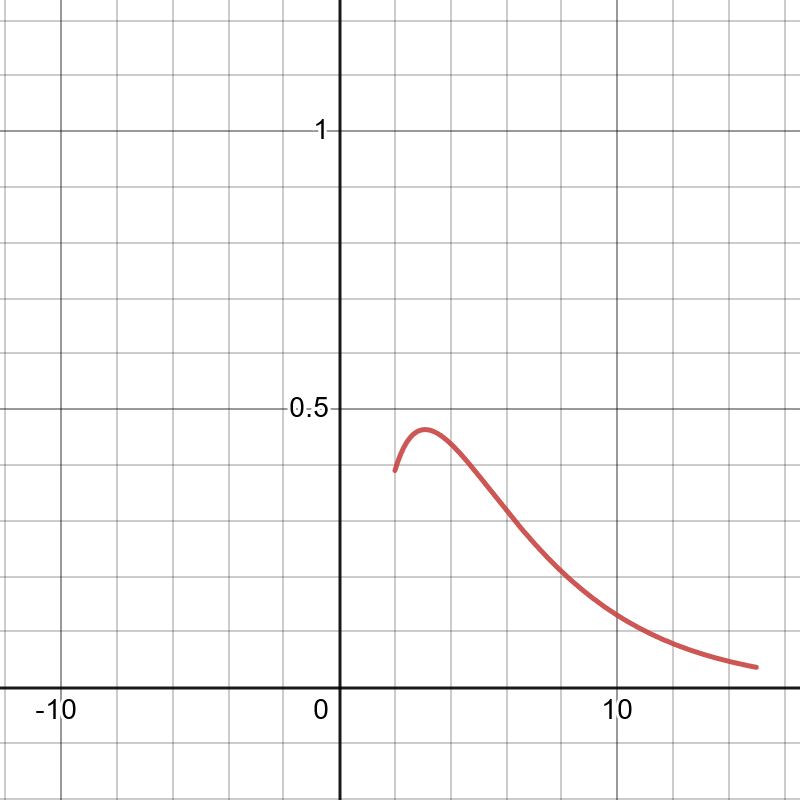
\includegraphics[scale=0.1]{desmos-graph(64).png}
    \end{solution}


\part [1] Use Desmos to graph $y = \frac{F(x+1)}{F(x)}$ for $ 2 \leq x \leq  15$. Reproduce the graph here. Based on the graph, what is your
guess for the numeric value of $\displaystyle   \lim_{x \to \infty}   \frac{F(x+1)}{F(x)} $?

    \begin{solution}[1.50in] We have $\frac{F(x+1)}{F(x)} = \frac{3}{4} \frac{\ln(x+1)}{\ln(x)}$.  The graph indicates
    that $\displaystyle   \lim_{x \to \infty}   \frac{F(x+1)}{F(x)} \approx 0.78$
    
    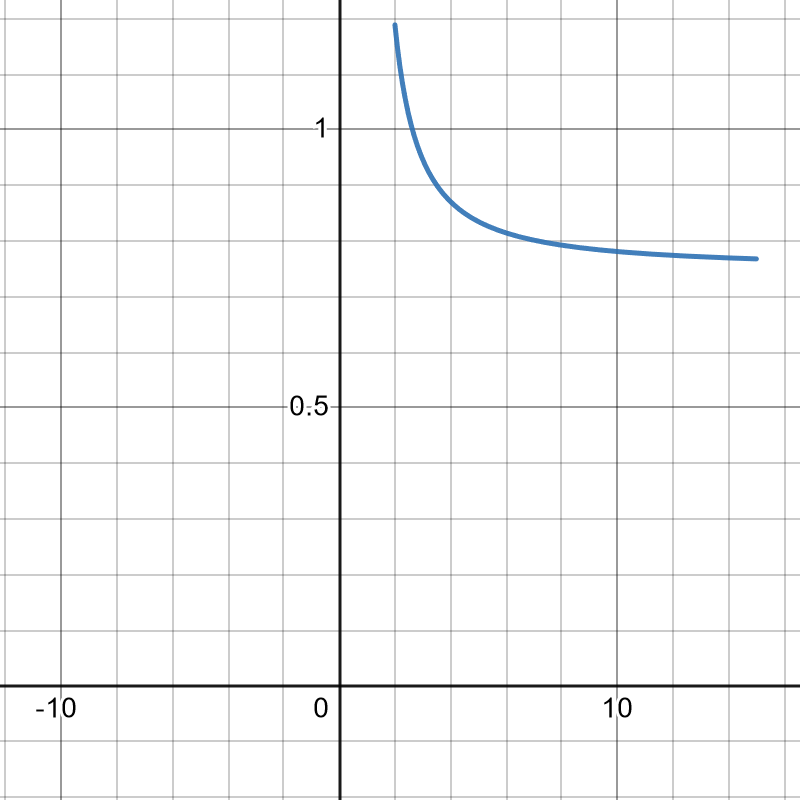
\includegraphics[scale=0.1]{desmos-graph(65).png}
        
    \end{solution}


\part [1] Use the l'H\^opital rule to find the numeric value of $\displaystyle   \lim_{x \to \infty}   \frac{F(x+1)}{F(x)} $.

   \begin{solution}%[1.50in]
   
   \begin{align*}  
    \lim_{x \to \infty}   \frac{3}{4} \frac{\ln(x+1)}{\ln(x)} &=   \lim_{x \to \infty} \frac{3}{4} \frac{\frac{1}{x+1}} {\frac{1}{x}}, \\
        &= \lim_{x \to \infty} \frac{3}{4} \frac{x}{x+1}, \\
        &= \frac{3}{4}.
   \end{align*}
        
    \end{solution}
    
\newpage


\part [1] Use the \emph{ratio test} to determine if the series $\displaystyle \sum_{k=2}^\infty F(k)$ converges or diverges.

   \begin{solution}[2.750in]
        Since $\displaystyle  \lim_{x \to \infty}   \frac{3}{4} \frac{\ln(x+1)}{\ln(x)} \in [0,1)$, the series $\displaystyle \sum_{k=2}^\infty F(k)$ converges.
    \end{solution}
    
\end{parts}
    
\question Use the \emph{ratio test} to determine if each series
converges or diverges.

\begin{parts}

    \part [1] $\displaystyle \sum_{k=0}^\infty \frac{2^k}{3^k +8}$

    \begin{solution}%[3.0in]
    \begin{align*}
       \lim_{k \to \infty} \frac{2 \left( {{3}^{k}}+8\right) }{{{3}^{k+1}}+8} &=
        \lim_{k \to \infty} \frac{2 \ln(3) 3^k}{ \ln(3) 3^{k+1}}, \\
        &= \lim_{k \to \infty} \frac{2}{3},\\
        &= \frac{2}{3}.
     \end{align*}
        
    \end{solution}

   
   \newpage
  

    \part [1] $\displaystyle \sum_{k=0}^\infty \frac{ ((k)!)^3}{(3 k)!} 14^k$

    \begin{solution}[4.50in]
    \begin{equation*}
     \lim_{k \to \infty}  \frac{14 {{\left( k+1\right) }^{2}}}{3 \left( 3 k+1\right) \, \left( 3 k+2\right) }
     = \frac{14}{27}.
    \end{equation*}
    So $\sum_{k=0}^\infty \frac{ ((k)!)^3}{(3 k)!} 14^k$ converges.
        
    \end{solution}
        
   
\end{parts}


\question [1] Find the numeric value of the $\displaystyle \lim_{k \to \infty} \frac{ ((k)!)^3}{(3 k)!} 14^k$.  Justify your answer.

Since  $\sum_{k=0}^\infty \frac{ ((k)!)^3}{(3 k)!} 14^k$ converges, we have  $\displaystyle \lim_{k \to \infty} \frac{ ((k)!)^3}{(3 k)!} 14^k = 0$.
\end{questions}
\end{document}
